\documentclass[tikz,border=8pt]{standalone}
\usepackage{braket}

\begin{document}
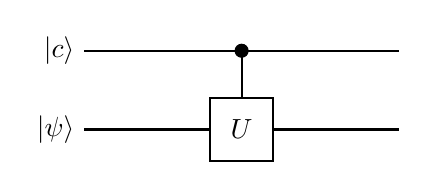
\begin{tikzpicture}[
  wire/.style={line width=0.8pt},
  gate/.style={draw,fill=white,line width=0.8pt,
    minimum width=0.8cm,minimum height=0.8cm,inner sep=0pt},
  control/.style={circle,fill=black,inner sep=1.8pt}
]
  \draw[wire] (0,1) -- (4,1);
  \draw[wire] (0,0) -- (4,0);
  \node[left] at (0,1) {$\ket{c}$};
  \node[left] at (0,0) {$\ket{\psi}$};
  \draw[wire] (2,0) -- (2,1);
  \node[control] at (2,1) {};
  \node[gate] at (2,0) {$U$};
\end{tikzpicture}
\end{document}
